\documentclass[parskip=full]{scrartcl}

\usepackage[utf8]{inputenc} % use utf8 file encoding for TeX sources
\usepackage[T1]{fontenc} % avoid garbled Unicode text in pdf
\usepackage[german]{babel} % german hyphenation, quotes, etc
\usepackage{hyperref} % detailed hyperlink/pdf configuration
\hypersetup{ % ‘texdoc hyperref‘ for options
pdftitle={Lamb.da - Das Spiel}
}
\usepackage{csquotes} % provides \enquote{} macro for "quotes"
\usepackage{graphicx}
\usepackage{float}
\usepackage{geometry}
\usepackage{enumerate}

\title{Lamb.da - Das Spiel}
%\date{October 12, 123}
\author{Name, Name, Name}

\begin{document}

\maketitle

\tableofcontents

\section{Einleitung}

Die Applikation "`Lambd.da"' soll Kindern im Grundschulalter auf eine spielerische Art und Weise die wesentlichen Aspekte des untypisierten Lambda-Kalküls und damit auch die Grundlage der funktionalen Programmierung vermitteln. In unserer Entwurfsdokumentation beschreiben und modellieren wir unsere Entwurfsentscheidungen und präsentieren dabei auch die Softwarearchitektur unserer Applikation.

Zunächst beschreiben wir die Funktionen der Applikation, die sich während der Entwurfsphase erst herauskristallisiert haben und deshalb noch nicht im Pflichtenheft erwähnt wurden. Anschließend wird erwähnt, welche der im Pflichtenheft genannten Wunschkriterien nicht mehr umgesetzt werden, da sich bereits in der Entwurfsphase ergab, dass wir diese nicht umsetzen können aus verschiedenen Gründen.

Im Kapitel Grobentwurf erläutern wir dann die von uns gewählten Designentscheidungen wie beispielsweise die eingesetzten Entwurfsmusters und beschreiben die Grobstruktur unserer Klassenpakete. Der Hauptteil und dabei auch der umfassendste Teil unseres Entwurfsdokuments bildet jedoch das Kapitel Feinentwurf mit unserer Klassendokumentation, in der alle Klassen und deren Methoden sowie deren Attribute und mögliche auftretende Exceptions aufgelistet und beschrieben werden. Es werden auch unsere eigenen verwendeten Interfaces beschrieben. Passend dazu fügen wir noch UML-Klassendiagramme zu diesem Entwurfsdokument an, in denen unsere beschriebenen Klassen und deren Komponenten als auch die Beziehungen zwischen den Klassen modelliert werden.

Des Weiteren Erläutern wir im Kapitel Datenstrukturen, wie die dauerhaft zu speichernden, logischen Komponenten unserer Applikation gespeichert und verwaltet und unsere Assets wie die Level des Spiels geladen werden. Wichtige Programmabläufe und die daraus resultierende Interaktion der Klassen untereinander werden durch UML-Sequenzdiagramme im Kapitel dynamische Diagramme beschrieben.
\section{Spielaufbau}

\subsection{Spielelemente}

Das Spiel ist in mehrere Level eingeteilt, welche jeweils ein zu lösendes Problem darstellen. Dabei muss der Spieler die zur Verfügung stehenden Spielelemente so anordnen, dass sie die Zielkriterien erfüllen. Es gibt folgende Spielelemente:

\begin{description}
\item[Lamm mit Zauberstab] repräsentiert die Abstraktion im $\lambda$-Kalkül. Die Farbe des Lamms $($nicht weiß$)$ beschreibt dabei den durch die Abstraktion gebundenen Variablennamen. Jedes Lamm besitzt eine Anzahl Edelsteine in derselben Farbe, außerdem hat es befreundete Lämmer in anderen Farben. Alle Edelsteine und Freunde eines Lamms werden vertikal unter diesem dargestellt. Ein Lamm kann sowohl eigene Edelsteine besitzen als auch solche anderer Lämmer aufbewahren.
\item[Lamm ohne Zauberstab] repräsentiert eine Klammerung im $\lambda$-Kalkül. Die Farbe dieses Lamms ist immer weiß. Lämmer ohne Zauberstab können keine Edelsteine besitzen, aber solche anderer Lämmer aufbewahren. Befreundete Lämmer und aufbewahrte Edelsteine werden auch vertikal unter dem weißen Lamm dargestellt. Weiße Lämmer, die nicht mehr gebraucht werden, verabschieden sich vom Spiel und verschwinden $($1./2. Regel für Lämmer ohne Zauberstab$)$.
\item[Edelstein] repräsentiert eine Variable im $\lambda$-Kalkül. Die Farbe des Edelsteins $($nicht weiß$)$ beschreibt dabei den Variablennamen. Edelsteine können entweder keinem oder genau einem Lamm gehören und von anderen Lämmern als dem Besitzer aufbewahrt werden.
\item[Freundeskreis] ist eine Gruppe von Spielelementen. Der Freundeskreis eines Lamms setzt sich aus allen von diesem Lamm aufbewahrten Edelsteinen sowie befreundeten Lämmern und deren Freundeskreisen zusammen.
\end{description}

\subsection{Spielregeln}

Die Spielregeln beschreiben die Art und Weise, wie eine Anordnung von Spielelementen umgewandelt werden kann. 

\begin{description}
\item[Verzauberungsregel] repräsentiert die $\beta$-Reduktion. Ein Lamm mit Zauberstab verzaubert den Freundeskreis, der sich vor ihm befindet. Dabei verwandelt er alle seine Edelsteine in den genannten Freundeskreis. Der ursprüngliche Freundeskreis verschwindet und das zaubernde Lamm verliert sowohl seinen Zauberstab als auch seine Farbe, erhält deshalb die Farbe weiß.
\item[Farbenregel] repräsentiert die $\alpha$-Konversion. Wenn ein Lamm einen Freundeskreis verzaubert und es dabei im eigenen sowie im verzauberten Freundeskreis zwei Elemente mit derselben Farbe gibt, wird vor Anwenden der Verzauberungsregel diese Farbe im zweiten Freundeskreis in eine andere noch nicht benutzte Farbe umgewandelt. Dabei müssen alle umgewandelten Spielelemente die gleiche neue Farbe erhalten.
\item[1. Regel für Lämmer ohne Zauberstab] repräsentiert die Klammerung um eine einzige Abstraktion oder Variable. Wenn ein Lamm ohne Zauberstab nur noch genau einen direkten Freund hat und keine Edelsteine aufbewahrt oder keinen Freund hat und genau einen Edelstein aufbewahrt, verabschiedet sich das Lamm vom Spiel und verschwindet. Dabei wird es durch den aufbewahrten Edelstein oder durch den einzigen direkten Freund inklusive dessen Freundeskreis ersetzt.
\item[2. Regel für Lämmer ohne Zauberstab] repräsentiert die Linksassoziativität von $\lambda$-Applikationen. Wenn ein Lamm ohne Zauberstab der erste Freund vor allen aufbewahrten Edelsteinen eines anderen Lammes ist, verabschiedet sich das Lamm vom Spiel und verschwindet. Dabei wird es durch seinen Freundeskreis ersetzt.
\item[Reihenfolge der Regelausführung] \hfill
\begin{enumerate}
\item Führe 1. und 2. Regel für Lämmer ohne Zauberstab solange aus, bis sie nicht mehr angewandt werden können.
\item Führe Verzauberungsregel $($inklusive Farbenregel falls nötig$)$ aus, wenn diese angewandt werden kann. Falls die Regel ausgeführt wurde, gehe zu Schritt 1.
\item Die Umwandlung ist abgeschlossen.
\end{enumerate}
\end{description}

\subsection{Spielmodi}

\begin{description}
\item[Editormodus] \hfill \\ Hier hat der Spieler die Möglichkeit Lämmer und Edelsteine in eine bestimmte Anordnung zu bringen. Durch das Level können dabei bestimmte Einschränkungen vorgegeben sein, z.B. bereits platzierte Spielelemente, begrenzte Anzahl von Spielelementen sowie benutzbaren Farben.
\item[Reduktionsmodus] \hfill \\ Hier wird eine bestimmte, gegebene Anordnung von Spielelementen gemäß den Spielregeln umgewandelt. Der Spieler hat die Möglichkeit die Reduktions-Schritte einzeln oder automatisch per Abspielmodus auszuführen zu lassen. Außerdem kann er einzelne Schritte rückgängig machen.
\end{description}

\subsection{Leveltypen}

\begin{description}
\item[Eingabe-Bestimmung] \hfill \\ Das Ziel des Spielers ist es einen Eingabe-Term im Editormodus zu finden, welcher durch Ausführen  der Spielregeln im Reduktionsmodus in den im Level gegebenen Ausgabe-Term umgewandelt werden kann. Falls die Reduktion nach einer begrenzten Anzahl von Schritten nicht terminiert, gilt das Level als nicht bestanden.
\item[Ausgabe-Bestimmung] \hfill \\ Das Ziel des Spielers ist es einen Ausgabe-Term im Editormodus zu finden, welcher durch Ausführen  der Spielregeln im Reduktionsmodus aus einem im Level gegebenen Eingabe-Term hervorgeht. Um im Reduktionsmodus nicht die Lösung des Levels zu verraten, kann hier nur eine Level-spezifische Anzahl von Reduktions-Schritten ausgeführt werden.
\end{description}

\section{Zielbestimmung}

	Das Produkt vermittelt Grundschülern auf spielerische Art und Weise das Konzept des untypisierten $\lambda$-Kalküls und dadurch die Grundlage funktionaler Programmierung   			    

\subsection{Musskriterien}

\begin{itemize}
	\item Bedienen über ein Smartphone per Toucheingabe
	\item Auflösen von Lamm-Konstellationen(Analogie zu $\lambda$-Termen)
	\begin{itemize}
		\item Bestimmen eines Endresultats bei einer bereits gegebenen, vollständigen Anordnung von Lämmern 
		\item Vervollständigen einer Anordnung von Lämmern, um ein gegebenes Endresultat zu erreichen
	\end{itemize}
	\item Verfolgen des Lernfortschritts durch Eltern oder Lehrer
	\begin{itemize}
		\item Achievementsystem
		\item Statistik
	\end{itemize}
	\item Aufrechterhaltung der Langzeitmotivation des Spielers
	\item Interaktive und intuitive Einführung zur Erklärung des Spiels und seiner Modi
\end{itemize}

\subsection{Wunschkriterien}

\begin{itemize}
	\item Für Tablets angepasste Version
	\item Spiel als Desktop-Anwendung
	\begin{itemize}
		\item Windows-Anwendung
		\item Mac OS X-Anwendung
	\end{itemize}
	\item Erstellen, Konfigurieren und Löschen von mehreren Spielerprofilen
	\item Anzeigen von Hinweisen zur Lösung des Level-Ziels
	\item Freier Modus, in dem eigene Level erstellt und simuliert werden können
	\item Belohnungen für das erstmalige Lösen der Level
	\item Eintauschen von Belohnungen gegen höherwertige Belohnungen in einem In-Game-Shop
	\item Option für Farbenblinde, durch die Farbenblinde Hilfestellungen beim Spiel bekommen
	\item Lehreroption, durch die die richtigen $\lambda$-Terme beim Abspielen der Level angezeigt werden
	\item Vermittlung einer kindergerechten Hintergrundgeschichte mittels Animationen
	\item Englisch als unterstütze Sprache
	\item Französisch als unterstütze Sprache
	\item Optionale Ausführung von unterschiedlichen Reduktionsstrategien bei der $\beta$-Reduktion von Lamm-Konstellationen (Normalreihenfolge ist die Standard-Reduktionsstrategie)
	\begin{itemize}
		% Kennt jemand davon den deutschen Fachausdruck?
		\item Applicative Order
		\item Call-By-Name
		\item Call-By-Value
	\end{itemize}
		
\end{itemize}

\subsection{Abgrenzungskriterien}

\begin{itemize}
	\item Keine direkte Bezugnahme zur funktionalen Programmierung oder dem $\lambda$-Kalkül (außer bei aktivierter Lehreroption) 
	\item Keine Unterstützung von Online-Funktionen
	\item Kein Mehrspielermodus
\end{itemize}

\section{Produkteinsatz}

	Das Produkt dient als Android-Lernapp für Grundschüler.
	
\subsection{Anwendungsbereiche}
\begin{itemize}
	\item In der Primarstufe des Erziehungs- und Ausbildungsbereichs (Grundschule)
	\item Im Unterhaltungsbereich für Kinder im Alter von 8 bis 12 Jahren
\end{itemize}

\subsection{Zielgruppen}
	Die Hauptzielgruppe sind Grundschüler, die durch das Spiel die Grundkonzepte des $\lambda$-Kalküls kennenlernen. Eltern und Lehrer können durch das Spiel den Lernfortschritt verfolgen.

\subsection{Betriebsbedingungen}
	Das Produkt wird hauptsächlich in Gruppen oder individuell während des Unterrichts an Grundschulen benutzt, es kann jedoch auch unter den gleichen Bedingungen in der Freizeit genutzt werden.
\section{Produktumgebung}

\subsection{Software}
\begin{itemize}
	%4.2 evtl. ersetzen 
	\item Das Produkt wird für Android entwickelt und sollte auf allen Versionen ab 4.2 (4.2 oder höher) laufen.
\end{itemize}

\subsection{Hardware}
\begin{itemize}
	\item Das Programm ist für Smartphones und Tablets konzipiert
	%sonst noch irgendwas? Hardware-Anforderungen?
\end{itemize}

\section{Funktionale Anforderungen}

In den folgenden Kapiteln werden Anforderung, die den Wunschkriterien zugeordnet sind, mit einem "`+"' hinter der Identifikationsnummer markiert.

\subsection{Profile}

Profile ermöglichen das Nutzen des Programms durch mehrere Anwender auf demselben Gerät.

\begin{itemize}
\item /FA110/ Jeder Nutzer soll ein eigenes Profil anlegen können, welches eindeutig durch den Profil-Namen gekennzeichnet ist. 
\item /FA120/ Bei Programmstart wird das zu benutzende Profil ausgewählt oder ein neues Profil erstellt.
\item /FA130/ Die zu einem Profil gespeicherten Daten können nach Erstellen des Profils geändert werden.
\item /FA140/ Ein Profil kann nach dem Erstellen gelöscht werden.
\item /FA150/ Zu jedem Profil werden Spieleinstellungen, Spielfortschritt und Spielstatistik gespeichert.
\item /FA160/ Beim Auswählen eines Profils werden die dazu gespeicherten Daten automatisch geladen.
\item /FA170/ Nach dem Auswählen eines Profils wird der Nutzer durch eine profilspezifische Nachricht begrüßt.
\end{itemize}

\subsection{Spielmodi}

Im Editormodus werden Terme erstellt, angezeigt und bearbeitet.

\begin{itemize}
\item /FA210/ Durch Ziehen können Objekte sowohl von der Werkzeugleiste als auch vom Term ausgewählt werden.
\item /FA220/ Während ein Objekt ausgewählt ist, wird die aktuelle Stelle im Term, an der das Objekt platziert werden kann, farblich markiert.
\item /FA230/ Während ein Objekt ausgewählt ist, kann durch Loslassen des Zeigers das Objekt an der aktuellen Stelle im Term platziert werden.
\item /FA240/ Während ein Objekt ausgewählt ist, kann durch Loslassen des Zeigers über der Werkzeugleiste das Objekt gelöscht werden.
\item /FA250/ Neu hinzugefügte Objekte erhalten die Farbe weiß.
\item /FA260/ Durch Drücken eines Objektes wird ein Dialog-Fenster geöffnet, in dem eine neue Farbe für das Objekt ausgewählt werden kann.
\item /FA270/ Das Ändern der Position oder Farbe von durch ein Level vorgegebenen Objekten kann optional unterdrückt werden.
\item /FA280/ Ein Term wird gültig sobald er den Spielregeln entspricht, worauf man in den Reduktionsmodus wechseln kann.
\end{itemize}

Im Reduktionsmodus werden Terme schrittweise durch Beta-Konversionen reduziert.

\begin{itemize}
\item /FA310/ Konversionen können einzeln schrittweise ausgeführt werden.
\item /FA320/ Konversionen können einzeln schrittweise zurückgesetzt werden.
\item /FA330/ Konversionen können automatisch abgespielt werden bis ein minimaler Term erreicht ist oder der Nutzer das Abspielen beendet.
\end{itemize}

\subsection{Level}

Das Spiel ist in Level eingeteilt, welche vom Spieler nacheinander freigeschaltet und gelöst werden.

\begin{itemize}
\item /FA410/ Das Ziel des Leveltyps "`Eingabe-Bestimmung"' ist es, im Editormodus einen gültigen Term zu erstellen, welcher durch Konversionen im Reduktionsmodus in einen minimalen im Level vorgegebenen Term umgewandelt wird.
\item /FA420/ Das Ziel des Leveltyps "`Ausgabe-Bestimmung"' ist es, im Editormodus einen gültigen Term zu erstellen, welcher aus der Reduktion eines im Level vorgegebenen Terms hervorgeht.
\item /FA430/ Nur das erste Level ist nach Erstellung eines Profils freigeschaltet, durch Abschließen eines Levels wird das darauf folgende Level freigeschaltet.
\item /FA440/ Nach erfolgreichen Abschließen eines Levels hat der Spieler die Möglichkeit ins nächste Level oder ins Hauptmenü zu wechseln.
\item /FA450/ Nach erfolgreichen Abschließen eines Levels wird der Spieler durch ein Nachrichtenfenster über den Erfolg informiert.
\item /FA460/ Nach erstmaligem erfolgreichen Abschließen des letzten Levels wird dem Spieler durch ein Nachrichtenfenster zu seiner Leistung gratuliert.
\item /FA470/ Über das Levelauswahlmenü kann der Spieler seinen Level-Fortschritt beobachten und bereits freigeschaltete Level erneut spielen.
\item /FA480/ Die Level sind in verschiedene Schwierigkeitsstufen eingeteilt, welche durch Farbe und Hintergrundbild voneinander unterscheidbar sind.
\item /FA490+/ Der Spieler kann sich Tipps und Lösungsansätze zum aktuellen Level anzeigen lassen.
\end{itemize}

\subsection{Gamification}

Durch ein Belohnungssystem wird die Spiel- und Lernfreude der Nutzer gesteigert.

\begin{itemize}
\item /FA510+/ Das erstmalige Abschließen eines Levels wird mit einer Level-spezifischen Anzahl von Münzen belohnt.
\item /FA520+/ Im Shop kann der Nutzer gegen Eintausch von Münzen neue Sounds, Hintergrundbilder und Texturen freischalten.
\item /FA530+/ Vor dem Freischalten eines Elements im Shop wird der Spieler um eine Bestätigung gebeten.
\item /FA540+/ Im Shop freigeschaltete Elemente können dort durch ein Kontrollkästchen aktiviert werden. Standardmäßig werden gerade gekaufte Sounds oder Hintergrundbilder sofort aktiviert.
\item /FA550+/ Für bestimmte Leistungen werden Erfolgsnachrichten in einem Erfolgsmenü angezeigt. Folgende Erfolge sind mindestens möglich:
\begin{itemize}
\item Erstes Level geschafft.
\item Alle Level eines Schwierigkeitsgrades abgeschlossen.
\item Alle Level des Spiels beendet.
% TODO
\end{itemize}
\item /FA560+/ Im Ladebildschirm werden zur Unterhaltung des Nutzers Comic-artige Sprechblasen mit lustigen und interessanten Texten angezeigt.
\end{itemize}

\subsection{Eltern und Lehrer}

Statistiken und Optionen für Eltern und Lehrer geben diesen einen Einblick in den Lernfortschritt des Kindes.

\begin{itemize}
\item /FA610/ In einem Statistikmenü werden verschiedene Daten angezeigt. Folgende Daten sind mindestens möglich:
\begin{itemize}
\item Spielzeit
\item Anzahl Versuche gesamt
\item Erfolgsquote für das Bestehen der Level
\item Häufigkeit der Nutzung von Hinweisen
% TODO
\end{itemize}
\item /FA620+/ Über den Lehrermodus wird im Editor- sowie im Reduktionsmodus der aktuelle Lambda-Term in mathematischer Darstellung angezeigt.
\item /FA630+/ Im Farbenblindenmodus, werden Objekte im Spiel mit verschiedenen Muster und Graustufen dargestellt, um das Spielen für Farbenblinde zu ermöglichen.
\end{itemize}

\subsection{Benutzerinteraktion}

\begin{itemize}
\item /FA710/ Über den Touchscreen des Gerätes kann der Nutzer mit dem Programm interagieren.
\item /FA720/ Über den Lautstärkeregler des Gerätes oder im Optionsmenü kann die Lautstärke des Programms verändert werden.
\item /FA730/ Mit dem "`Zurück-Knopf"' des Gerätes kann von einem Menü in das vorherige Menü gewechselt werden.
\item /FA740/ Mit der Drag\&Drop-Geste kann im Editormodus der Term auf dem Bildschirm verschoben werden.
\item /FA750+/ Mit die Pinch-Geste kann im Editormodus die Zoomstufe verändert werden.
\item /FA760/ Über ein Kontrollkästchen im Hauptmenü kann die Hintergrundmusik an- und ausgeschaltet werden.
\item /FA770+/ Das Programm unterstützt das Auswählen der Sprachen Englisch, Deutsch und Französisch.
\end{itemize}

\section{Produktdaten}
% TODO L und LD Nummern anpassen

Alle Daten werden Profil-spezifisch gespeichert.

\begin{itemize}

\item /D10/ Profil
\begin{itemize}
\item /LD11/ Profilname
\item /LD12/ Avatar
\item /LD13/ Sprache
\end{itemize}

\item /D20/ Spieloptionen
\begin{itemize}
\item /LD21/ Lehrermodus aktiviert
\item /LD22/ Hintergrundmusik aktiviert
\end{itemize}

\item /D30/ Spielfortschritt
\begin{itemize}
\item /LD31/ Letztes freigeschaltetes Level
\item /LD32/ Abgeschlossene Achievements
\end{itemize}

\item /D40/ Statistik
\begin{itemize}
\item /LD41/ Gesamtanzahl der Versuche
\item /LD42/ Erfolgreiche Versuche
\item /LD43/ Zeit im Editor-Modus verbracht
\item /LD44/ Zeit im Reduktions-Modus verbracht
\item /LD45/ Gesamtzeit im Programm verbracht
\item /LD46/ Anzahl der genutzten Hinweise
% TODO
\end{itemize}

\end{itemize}
\section{Nichtfunktionale Anforderungen}

\subsection{ProduktLeistungen}

\begin{itemize}
\item /NF110/ Das Spiel soll Android 4.2 und Höher unterstützen
\item /NF120/ Die Ladezeit des Spiels darf 15 SeKunden nicht über­schrei­ten 
\item /NF130/ Der Übergang zwischen Levels dauert höchstens 10 SeKunden.
\item /NF140/ Das Spiel Stürtzt maximal 1 mal pro Monat ab 
\item /NF150/ Das Abstürtzen des Spiels führt nicht zum Verlust der gespeicherte daten (Geschafte Levels,Verdiente Coins , Gekaufte Hintergründe und Sounds ... )
\item /NF160/ Der übergang zwischen levels  darf 5 Secunden nicht über­schrei­ten
\end{itemize}


\subsection{Benutzungschnittstelle}
\begin{itemize}
\item /NF210/ Das Spiel soll für Grundschülkinder verständlich und leicht zu bedienen sein
\item /NF215/ Es werden möglichst viele Symbole und wenig Text benutzt 
\item /NF220/ Das Spiel  muss kindern Spass machen und Lambda-Kalkül Konzepte beibrigen   
\end{itemize}


\subsection{Rechtliches}
\begin{itemize}
\item /NF310/ Das Spiel hat kein Zugriff auf die Daten des Bentzers (Standort,Kontakte,Fotos,unsw...)
\item /NF320/ Das Spiel darf keine externe Datenbanken für  das Speichern der Stastiken  verwenden, bzw. die Statistiken nicht für komerziele Zwecken verwenden  
\item /NF330/ Das Spiel  entspricht die Datenschutzrichtlinien der Bundesdatenschutzgestzes  (BDSG)
\item /NF340/ Das Spiel wird nicht  Kommerzialisiert
\item /NF350/ Das Spiel Benutzt nur frei Grfics und Songs
\end{itemize}
\section{Anwendungsfälle und Szenarien}

\subsection{Szenarien}

\subsubsection{Erstausführung}
\paragraph{Erstmaliges Starten der Application}
\begin{itemize}
	\item Der Benutzer startet erstmalig die Application.
	\item Es wird ein Ladebildschirm angezeigt.
	\item Der Benutzer wird automatisch in die Sequenz zur Erstellung eines Profils weitergeleitet. (Siehe Szenario "`Profil anlegen"')
	\item Das soeben angelegte, erste Profil wird automatisch aktiviert und der Benutzer wird ins Hauptmenü des Spiels weitergeleitet.
	\item Durch drücken des Buttons "`Start"' wird ein erstes Spiel gestartet.
	\item Alternativ stehen dem Benutzer auch alle anderen Funktionen des Hauptmenüs zur Verfügung.
\end{itemize}
\paragraph{Erstes Spiel starten}
\begin{itemize}
	\item Das Spiel überspringt die Levelauswahl und startet gleich mit dem ersten Level (Tutoriallelvel).
	\item Die Hintergrundgeschichte des Spiels wird dem Benutzer innerhalb einer Sequenz erklärt.
	\item Das Spiel startet im Editormodus.
	\item Die wichtigsten Bedienflächen werden schrittweise und nacheinander erklärt (Tutorial).
	\item Das Ziel des Levels wird als Popup angezeigt.
	\item Der Benutzer muss nun zur Erfüllung des Levelziels die im Tutorial erwähnten Buttons und Dialoge benutzen.
	\item Ist dies geschehen, so ist das Tutoriallevel beendet und der Levelabschluss-Dialog erscheint.
	\item Der Benutzer erhält eine Belohnung und kann nun wahlweise entweder das soeben gespielte Level erneut spielen, zum nächsten Level fortschreiten oder zurück ins Hauptmenü des Spiels gehen.
\end{itemize}

\subsubsection{Level spielen}
\paragraph{Voraussetzungen}
\begin{itemize}
	\item Der Benutzer hat bereits ein Spielerprofil angelegt.
	\item Der Benutzer befindet sich zu Beginn im Hauptmenü.
\end{itemize}
\paragraph{Levelauswahl und -start}
\begin{itemize}
	\item Im Hauptmenü kann der Benutzer im aktuell ausgewählten Profil sein aktuelles Level (das höchste, noch nicht erfolgreich bestandene Level) durch drücken des Buttons "`Start"' direkt starten.
	\item Alternativ wird der Benutzer durch drücken des Buttons "Level" in das Levelauswahlmenü weitergeleitet.
	\item Das Levelauswahlmenü ist als Raster von nummerierten Buttons angeordnet, wobei ein nummerierter Button einem Level entspricht.
	\item Die Höhe der Nummerierung sowie die Farbe des Buttons kennzeichnen den Schwierigkeitsgrad des Levels.
	\item Die Level werden durch drücken des jeweiligen Buttons gestartet.
	\item Ein Level lässt sich erst starten, wenn alle vorherigen Level erfolgreich abgeschlossen wurden.
	\item Am Anfang eines Levels kann es in Folge eines Tutorials zu einer Sequenz kommen, die gegebenenfalls übersprungen werden kann.
	\item Das Levelziel wird als Popup eingeblendet und kann über einen Button im Spiel jederzeit erneut eingesehen werden.
	\item Ein Level startet im Editormodus.
\end{itemize}
\paragraph{Editormodus}
\begin{itemize}
	\item Nach Anzeigen des Levelziels wird auf dem Bildschirm der aktuelle Zustand des Spielfelds angezeigt.
	% besserer Begriff als Editorleiste ?
	\item Zur Ergänzung des Spielfelds und zum Erreichen des Levelziels lassen sich einzelne Spielelemente aus einer Editorleiste per Drag$\&$Drop auf dem Spielfeld platzieren (bei höheren Level).
	\item Beim Platzieren per Drag$\&$Drop werden Platzierungflächen als Hilfe zur geeigneten Absetzung der Elemente hervorgehoben.
	\item Zum Entfernen von Spielelementen aus dem Spielfeld werden die 
	\item Beim Drücken auf ein Spielelement (Lamm oder Edelstein) öffnet sich ein Farbauswahldialog mit acht Farben.
	\item Nachdem der Benutzer ein Farbe ausgewählt hat, färbt sich das entsprechende Spielelement in dieser Farbe und der Farbauswahl-Dialog schließt sich.
	\item Zum Entfernen von Spielelementen aus dem Spielfeld können die jeweiligen Spielelemente ebenfalls per Drag$\&$Drop in die Editorleiste zurückgelegt werden.
	\item Durch das Drücken des Hinweisbuttons wird dem Benutzer ein Lösungsansatz zum erreichen des Levelziels als Popup angezeigt.
	\item Durch des Drücken des Pausierbuttons wird der Pausen-Dialog aufgerufen.
	\item Im Pausen-Dialog lässt sich das Level durch das Drücken des jeweiligen Buttons wahlweise entweder fortsetzen oder in seinen Anfangszustand zurücksetzen oder es kann zum Haupt- oder Levelauswahlmenü zurückgekehrt werden.
	\item Der Reduktionsmodus ist über ein "`Weiter"'-Button erreichbar. 
	\item Es lässt sich erst zum Reduktionsmodus wechseln, wenn alle Spielelemente auf dem Spielfeld eingefärbt sind.
\end{itemize}

\paragraph{Reduktionsmodus}
\begin{itemize}
	\item Der Benutzer befindet sich nun im Reduktionsmodus.
	\item Das Spielfeld befindet sich in dem Zustand, der im Editormodus erstellt wurde.
	\item Gemäß den Spielregeln wird die Anordnung von Spielelementen auf dem Spielfeld reduziert.
	\item Alle Reduktionsschritte werden auf dem Spielfeld dargestellt.
	\item Es ist wahlweise eine vollständige, automatische Reduktion oder eine schrittweise Reduktion möglich.
	\item Die automatische Reduktion wird vom Benutzer durch das Drücken eines Start-/Fortsetzung-Button und eines Pausierbuttons gesteuert.
	\item Die schrittweise Reduktion wird vom Benutzer durch das Drücken eines Vorwärts-oder eines Rückwärts-Buttons gesteuert.
	\item Der Vorgang läuft solang bis gemäß der gewählten Reduktionsstrategie die Anordnung nicht mehr weiter reduziert werden kann.
	\item Dann wird überprüft, ob das Levelziel erreicht wurde.
	\item Anschließend erscheint der Levelabschluss-Dialog, der den Benutzer darüber informiert, ob dieser das Level erfolgreich abgeschlossen hat oder nicht.
	\item Beim erstmaligen erfolgreichen Bestehen des Levels erhält der Benutzer eine Belohnung, die im Levelabschluss-Dialog ebenfalls angezeigt wird.
	\item Nun kann der Benutzer noch wahlweise durch das Drücken des jeweiligen Buttons das soeben gespielte Level erneut spielen, zum nächsten Level fortschreiten (nur bei einem erfolgreichen Abschluss des Levels) oder zurück ins Hauptmenü des Spiels gehen.
\end{itemize}

\subsubsection{Profil anlegen}
\paragraph{Voraussetzungen}
\begin{itemize}
	\item Der Benutzer befindet sich im Szenario "`Erstausführung"' oder er drückt auf den Button zum hinzufügen von neuen Profilen oder er drückt auf den Einstellungsbutton neben einem vorhanden Profil im Profilauswahlmenü.
\end{itemize}
\paragraph{Profilanlegung}
\begin{itemize}
	\item Der Benutzer wählt im ersten Dialogfenster seine Sprache.
	\item Die voreingestellte Sprache lässt sich über die Pfeil-Buttons ändern.
	\item Über den "`Weiter"'-Button gelangt der Benutzer zum nächsten Dialogfenster, in dem er nach seinem Namen gefragt wird.
	\item Durch das Drücken auf das Eingabefeld öffnet sich die Eingabemethode.
	\item Der Benutzer gibt seinen Namen ein.
	\item Falls das Eingabefeld noch leer ist oder falls der Name bereits für ein anderes Profil vorhanden ist, so bleibt der "`Weiter"'-Button deaktiviert.
	\item Bei gültiger Eingabe eines Namens kann der Benutzer zum Avatarauswahlfenster wechseln.
	\item In diesem Dialogfenster kann der Benutzer aus einer vorgegebenen Auswahl von Avatarbildern mittels Pfeil-Button wählen.
	\item Mittels der "`Zurück"'- und "`Weiter"'-Buttons können nochmals die Einstellungen des Profils bearbeitet werden oder das Profil kann durch das Drücken des Bestätigungsbuttons fertig gestellt werden.
	\item Dem Benutzer erscheint nun automatisch ein Popup zur Begrüßung, auf dem sein Profilname und sein gewähltes Avatarbild angezeigt wird.
	\item Das neue Profil wird automatisch aktiviert und der Benutzer wird zum Hauptmenü weitergeleitet.
	\item Das Profil wird im Hauptmenü als Button dargestellt.
\end{itemize}

\subsubsection{Profilverwaltung}
\paragraph{Voraussetzungen}
\begin{itemize}
	\item Der Benutzer besitzt ein Spielerprofil.
	\item Der Benutzer befindet sich zu Beginn im Hauptmenü.
\end{itemize}
\paragraph{Neues Profil anlegen}
\begin{itemize}
	\item Der Benutzer drückt im Hauptmenü auf den Profilbutton, wodurch das Profilauswahlmenü erscheint.
	\item Im Profilauswahlmenü werden alle bereits erstellte Profile mit Namen und Avatar angezeigt.
	\item Der Benutzer drückt im Profilauswahlmenü auf den Button zum Hinzufügen von neuen Profilen.
	\item Der Benutzer wird nun zur Profilanlegungs-Sequenz des Szenarios "`Profil anlegen"' weitergeleitet.
	\item Anschließend befindet sich der Benutzer mit seinem neuen Profil wieder im Hauptmenü.
\end{itemize}
\paragraph{Profil konfigurieren}
\begin{itemize}
	\item Der Benutzer drückt im Hauptmenü auf den Profilbutton, wodurch das Profilauswahlmenü erscheint. 
	\item Im Profilauswahlmenü drückt der Benutzer auf den Einstellungsbutton neben den entsprechenden Profil, das er konfigurieren will. 
	\item Der Benutzer wird nun zur Profilanlegungs-Sequenz des Szenarios "`Profil anlegen"' weitergeleitet (die bisherigen Einstellungen des Profils sind als Voreinstellungen gesetzt).
	\item Anschließend befindet sich der Benutzer mit seinem neu konfigurierten Profil wieder im Hauptmenü.
\end{itemize}

\subsubsection{Profil wechseln}
\paragraph{Voraussetzungen}
\begin{itemize}
	\item Es sind bereits mindestens zwei Profile angelegt worden.
	\item Der Benutzer befindet sich zu Beginn im Profilauswahlmenü.
\end{itemize}
\paragraph{Profil wechseln}
\begin{itemize}
	\item Der Benutzer drückt im Profilauswahlmenü auf das Profil, auf das er wechseln will.
	\item Der Benutzer wird automatisch mit seinem neuen Profil zum Hauptmenü weitergeleitet.
\end{itemize}

\subsubsection{Profil löschen}
\paragraph{Voraussetzungen}
\begin{itemize}
	\item Es sind bereits mindestens zwei Profile angelegt worden.
	\item Der Benutzer darf das Profil, das er löschen will, nicht aktiviert haben.
	\item Der Benutzer befindet sich zu Beginn im Profilauswahlmenü.
\end{itemize}
\paragraph{Profil löschen}
\begin{itemize}
	\item Der Benutzer drückt im Profilauswahlmenü auf den Löschbutton neben dem Profil, das er löschen will.
	\item Es erscheint ein Dialogfenster, in dem der Benutzer gefragt wird, ob er sich sicher ist, dass er dieses Profil löschen will.
	\item Verneint der Benutzer die Frage, dann bricht der Löschvorgang ab und der Benutzer befindet sich wieder im normalen Profilauswahlmenü.
	\item Falls der Benutzer den Vorgang bestätigt, erscheint ein Popup, das die Bestätigung des Löschvorgangs und das gelöschte Profil anzeigt.
	\item Der Benutzer wird nun automatisch zum aktualisierten Profilauswahlmenü weitergeleitet, in dessen Profilliste das soeben gelöschte Profil entfernt wurde.
\end{itemize}

\subsubsection{Einstellungen ändern}
\paragraph{Voraussetzungen}
\begin{itemize}
	\item Der Benutzer befindet sich zu Beginn im Hauptmenü.
\end{itemize}
\paragraph{Einstellungen ändern}
\begin{itemize}
	% Einstellungsbutton auch im Pausenmenü ?
	\item Der Benutzer drückt im Hauptmenü auf den Einstellungsbutton, was ihn zum Einstellungsmenü weiterleitet.
	\item Im Einstellungsmenü befinden sich
	\begin{itemize}
		\item Ein Ankreuzfeld zur Aktivierung des Lehrermodus.
		\item Ein Ankreuzfeld zur Aktivierung des Farbenblindenmodus.
		\item Ein Anzeigebutton für die Statistik.
		% Warum statt Ton nicht ein Geräusche-Schiebregler ?
		\item Ein Schieberegler für den Ton.
		\item Ein Schieberegler für die Hintergrundmusik.
	\end{itemize}
	\item Der Benutzer kann alle Einstellungen ändern bis er zufrieden mit ihnen ist.
	\item Die Toneinstellungen geben beim loslassen des Schiebereglers ein Testgeräusch von sich.
	\item Die Toneinstellungen sind relativ zur eigentlichen Medienlautstärke.
	\item Alle Änderungen an den Einstellungen werden sofort übernommen und global für alle Profile gespeichert.
	\item Durch das Drücken des Hilfsbutton erhält der Benutzer mehr Informationen zu den Einstellungsoptionen.
	\item Durch das Drücken des "`Zurück"'-Buttons gelangt der Benutzer zurück in sein vorheriges Menü.
\end{itemize}

\subsubsection{Belohnungen eintauschen}
\paragraph{Voraussetzungen}
\begin{itemize}
	\item Es existiert mindestens ein Spielerprofil.
	\item Der Benutzer befindet sich zu Beginn im Hauptmenü.
\end{itemize}
\paragraph{Belohnungen eintauschen}
\begin{itemize}
	\item Der Benutzer drückt im Hauptmenü auf den Button mit seinem aktuellen Münzstand, wodurch das Belohnungsmenü geöffnet wird.
	\item Die Belohnungen sind im Belohnungsmenü in die Kategorien Musik (Hintergrundmusik), Hintergründe (für Level) und Avatare (zusätzliche Avatare zur Auswahl bei der Profilerstellung) eingeteilt.
	\item Die Belohnungen werden durch das Bezahlen mit Münzen (die übliche Belohnung für das erstmalige bestehen eines Levels) gekauft und danach nach Belieben aktiviert.
	\item Es gibt pro Kategorie einen Button.
	\item Beim Drücken eines Kategoriebuttons wird eine Liste mit den einzelnen Belohnungen der Kategorie aufgeklappt.
	\item Beim erneuten Drücken des selben Kategoriebuttons wird die Kategorieliste wieder zugeklappt.
	\item Pro Belohnung in der Kategorieliste sind der Belohnungsname, die Kosten in Münzen sowie ein Ankreuzfeld für die mögliche Aktivierung nach einem Kauf aufgelistet.
	\item Falls der Benutzer nun eine Belohnung aus der Musik-Kategorie will, muss er zunächst den Musik-Kategoriebutton drücken.
	\item In der nun aufklappenden Musik-Kategorieliste wählt er eine Belohnung aus, für die er genügend Münzen besitzt.
	\item Nun öffnet sich ein Dialogfenster zur Bestätigung des Kaufs.
	\item Falls der Benutzer den Kaufvorgang bestätigt, wird die Bestätigung des Vorgangs in einem Popup angezeigt, falls nicht so wird der Kaufvorgang abgebrochen.
	\item Der neue Münzenstand wird nun im Belohnungsmenü angezeigt.
	\item Bereits gekaufte Belohnungen werden im Belohnungsmenü hervorgehoben.
	\item Belohnungen, die aufgrund des aktuellen Münzstandes nicht erworben werden können, werden nicht in einer Kategorieliste aufgelistet.
	\item Manche erworbene Belohnungen können nicht zur selben Zeit in einem Profil aktiviert sein, wie beispielsweise die Belohnungen der Musik-Kategorie.
	\item Durch das Drücken des "`Zurück"'-Buttons des Belohnungsmenüs kehrt der Benutzer wieder ins Hauptmenü zurück.
\end{itemize}

\subsubsection{Erfolgsansicht}
\paragraph{Voraussetzungen}
\begin{itemize}
	\item Es existiert mind. ein Spielerprofil.
	\item Der Benutzer befindet sich zu Beginn im Hauptmenü.
\end{itemize}
\paragraph{Erfolge ansehen}
\begin{itemize}
	\item Der Benutzer drückt den Button "`Erfolge"' im Hauptmenü, wodurch das Achievementmenü geöffnet wird.
	\item Die Erfolge sind im Achievementmenü in Kategorien eingeordnet.
	\item Jeder Erfolg wird auf einem Button dargestellt.
	\item Durch das Drücken eines bestimmten Buttons erscheint ein Popup, welches mehr Informationen zu dem entsprechenden Erfolg anzeigt.
	\item Bereits vom Spielerprofil freigeschaltene Erfolge sind hervorgehoben und aktiviert, noch nicht freigeschaltene Erfolge sind deaktiviert.
	\item Durch das Drücken des "`Zurück"'-Buttons kehrt der Benutzer ins Hauptmenü zurück.
\end{itemize}

\subsubsection{Level erzeugen im freien Modus}

\subsubsection{Betriebssysteminteraktion}
\begin{itemize}
	\item Der Benutzer befindet sich während des Spielens eines Levels in einem Spielmodus (Editormodus, Reduktionsmodus oder Freier Modus)
	\item Es kann nötig werden, das Spiel direkt ohne Umwege über Menüs zu verlassen.
	\item Dies kann bspw. bei der Betätigung des "`Home"'-Buttons  oder auch bei Betriebssystemereignissen geschehen.
	\item Die Application soll in diesem Fall den aktuellen Zustand, also die Anordnung der Spielelemente auf dem Spielfeld, abspeichern.
	\item Beim Neustart der Application soll es so möglich sein, die vorherige Konstellation der Spielelemente wiederherzustellen.
\end{itemize}

\section{Testfälle}
% TODO T Nummern anpassen


\subsection{Globale Testfälle}
Folgende Funktionssequenzen sind zu überprüfen:

\begin{itemize}
\item /T110/ Erstmaliges Starten des Programms
\begin{itemize}
\item Während das Programm sich im Ladebildschirm befindet, werden dem Spieler Comic-artige Sprechblasen mit lustigen und interessanten Texten angezeigt.
\item Der Nutzer startet das Programm und befindet sich im Sprachauswahlmenü $($Abb. \ref{fig:Sprachauswahlmenu}$)$. Mit den Sprachauswahl-Buttons $($S2$)$ wählt er die Sprache Deutsch aus.
\item Durch Drücken des Weiter-Buttons $($B1$)$ wechselt das Programm zum Namenswahlmenü $($Abb. \ref{fig:Namenswahlmenu}$)$. Hier wird der Spieler nach seinem Namen gefragt, den er in der Namenseingabe-Textbox eingibt.
\item Durch Drücken des  Weiter-Buttons $($B1$)$ wechselt das Programm zum Avatarauswahlmenü $($Abb. \ref{fig:Avatarauswahlmenu}$)$.
 Mit den Knöpfen A1 und A2 wählt er den gewünschten Avatar aus.
\item Durch Drücken des Weiter-Buttons $($B1$)$ erscheint der Begrüßungsbildschirm $($Abb. \ref{fig:Begrussungsbildschirm}$)$ mit Name und Avatar des Spielers.
\item Nach 3 Sekunden wechselt das Programm automatisch zum Hauptmenü $($Abb. \ref{fig:Hauptmenu}$)$.
\end{itemize}

\item /T120/ Starten des Programms, nachdem mindestens ein Profil bereits erstellt wurde
\begin{itemize}
\item Der Nutzer startet das Programm und befindet sich im Profilauswahlmenü $($Abb. \ref{fig:Profilauswahlmenu}$)$. Hier wählt er durch Drücken des Name-Button $($P1$)$, welcher mit seinem Namen beschriftet ist, sein Profil aus.
\item Es erscheint der Begrüßungsbildschirm $($Abb. \ref{fig:Begrussungsbildschirm}$)$ mit Name und Avatar des Spielers.
\item Nach 3 Sekunden wechselt das Programm automatisch zum Hauptmenü $($Abb. \ref{fig:Hauptmenu}$)$.
\end{itemize}

\item /T130/ Profildaten ändern
\begin{itemize}
\item Der Nutzer befindet sich im Profilauswahlmenü $($Abb. \ref{fig:Profilauswahlmenu}$)$.
\item Durch Drücken des Konfigurations-Buttons $($P2$)$ öffnet sich ein Dialog-Fenster, in dem der Nutzer die Option "`Profil editieren"' wählt. Das Programm wechselt zum Sprachauswahlmenü $($Abb. \ref{fig:Sprachauswahlmenu}$)$. 
\item Wie in /T110/ beschrieben gibt der Nutzer nacheinander Sprache, Namen und Avatar ein.
\item Nach Drücken des Bestätigungs-Buttons $($B3$)$ im Menü Avatarauswahlmenü $($Abb. \ref{fig:Avatarauswahlmenu}$)$ wechselt das Programm zurück in das Profilauswahlmenü $($Abb. \ref{fig:Profilauswahlmenu}$)$.
\end{itemize}

\item /T140/ Profil löschen
\begin{itemize}
\item Der Nutzer befindet sich im Profilauswahlmenü $($Abb. \ref{fig:Profilauswahlmenu}$)$.
\item Durch Drücken des Konfigurations-Buttons $($P2$)$ öffnet sich ein Dialog-Fenster, in dem der Nutzer die Option "`Profil löschen"' wählt.
\item In einem weiteren Dialog-Fenster bestätigt der Spieler seine Aktion.
\item Das Programm wechselt zurück in das Profilauswahlmenü $($Abb. \ref{fig:Profilauswahlmenu}$)$. Da das Profil jetzt gelöscht ist, erscheint es hier nicht mehr zur Auswahl.
\end{itemize}

\item /T150/ Einen Term im Editor-Modus bearbeiten
\begin{itemize}
\item Der Nutzer hat ein Level gestartet und befindet sich jetzt im Editor-Modus.
% Knops "Hinweis"
\item Durch Drücken des Knopfes TODO öffnet sich ein Popupfenster, in welchem dem Spieler ein Hinweis zur Lösung des aktuellen Levels gegeben wird.
\item Durch die Drag\&Drop Geste fügt er nacheinander sowohl ein weißes Lamm als auch ein weißer Edelstein zum aktuellen Term hinzu.
\item Durch Drücken des Lamms öffnet sich ein Kontextmenü, in dem der Spieler eine Farbe auswählen kann. Nach Drücken der gewünschten Option wechselt das Lamm seine Farbe.
\item Durch die Drag\&Drop Geste zum Werkzeugmenü entfernt der Spieler einen Edelstein aus dem Term.
\item Der Spieler versucht ein durch das Level bereits vorgegebenes Lamm durch die Drag\&Drop Geste zu verschieben, das Programm unterdrückt dies aber.
% Knopf "Play"
\item Der Term ist jetzt gültig und der Spieler drüct den Knopf TODO. Das Programm wechselt zum Reduktions-Modus.
\end{itemize}

\item /T150/ Einen Term im Reduktions-Modus konvertieren
\begin{itemize}
% Knopf "Play"
\item Der Nutzer hat nach Bearbeiten eines Terms im Editor-Modus den Knopf TODO betätigt und befindet sich jetzt im Reduktions-Modus.
% Knopf "Step forward"
\item Durch Drücken des Knopfes TODO wird der Term um einen Schritt reduziert.
% Knopf "Step backward"
\item Durch Drücken des Knopfes TODO wird der Term auf den Zustand vor dem letzten Schritt zurückgesetzt.
% Knopf "Play" "Pause"
\item Durch Drücken des Knopfes TODO werden automatisch einzelne Reduktionen nacheinander ausgeführt. Nach 3 Schritten drückt der Spieler den Knopf TODO und die Ausführung pausiert.
% Knopf "Step forward"
\item Durch Drücken des Knopfes TODO wird der Term um einen Schritt reduziert. Der Term ist jetzt minimal und gleich dem gewünschten Term, der durch das Level vorgegeben ist.
\item Ein Popup-Fenster wird geöffnet, in dem der Spieler darüber informiert wird, dass er das Level abgeschlossen hat.
\end{itemize}

\item /T160/ Level auswählen
\begin{itemize}
\item Der Nutzer befindet sich im Hauptmenü $($Abb. \ref{fig:Hauptmenu}$)$ und drückt den Level-Button $($H2$)$. Das Programm wechselt zum Levelauswahlmenü $($Abb. \ref{fig:Levelauswahlmenu}$)$.
\item Einige Level sind bereits abgeschlossen und durch einen Haken markiert, ein Level ist freigeschaltet und die restlichen Level nicht freigeschaltet und deshalb durch ein Schloss markiert. Level mit demselben Schwierigkeitsgrad sind hier farblich gleich gekennzeichnet.
\item Der Spieler wählt das erste Level durch Drücken des Levelstart-Buttons $($L1$)$ aus und das Programm wechselt in den Editor-Modus zur Bearbeitung dieses Levels.
\end{itemize}

\item /T170/ Das Einkaufsmenü benutzen
\begin{itemize}
\item Der Spieler besitzt durch Abschluss mehrerer Level eine Anzahl an Münzen. Bisher hat er noch keine Elemente im Shop gekauft.
\item Das Programm befindet sich im Hauptmenü $($Abb. \ref{fig:Hauptmenu}$)$. Durch Drücken des Einkaufs-Button $($H6$)$ wechselt es zum Einkaufsmenü $($Abb. \ref{fig:Einkaufsmenu}$)$.
\item Hier wählt der Spieler das Musik-Dropdownmenü $($E1$)$ aus. Es erscheinen mehrere zum Kauf verfügbare Objekte $($Abb. \ref{fig:Einkaufsmenu_Dropdown}$)$.
\item Der Spieler wählt den ersten Sound aus und wird darauf durch ein Dialog-Fenster zur Bestätigung des Kaufs gebeten.
\item Nach der Bestätigung wird der Sound freigeschaltet und automatisch aktiviert.
\item Durch Wiederholen dieser Schritte kauft er auch den zweiten verfügbaren Sound. Dieser wird automatisch aktiviert.
\item Der Spieler aktiviert nun wieder den ersten Sound, indem er auf das zweite Element drückt. Das aktivierte erste Element wird durch einen Haken gekennzeichnet, der Haken beim deaktivierten zweiten Element wird entfernt.
\end{itemize}

\item /T180/ Optionen auswählen
\begin{itemize}
\item Das Programm befindet sich im Hauptmenü $($Abb. \ref{fig:Hauptmenu}$)$. Durch Drücken der Stumm-Checkbox $($H5$)$ wird die Hintergrundmusik deaktiviert.
\item Durch Drücken des Optionen-Buttons $($H4$)$ wechselt das Programm in das Optionsmenü $($Abb. \ref{fig:Optionsmenu}$)$. Hier aktiviert der Spieler durch Drücken der Lehrermodus-Checkbox $($O1$)$ den Lehrermodus und durch Drücken der Farbenblindenmodus-Checkbox $($O2$)$ den Farbenblindenmodus.
\item Durch Verschieben des Geräusche-Sliders $($O4$)$ passt der Spieler die Geräuschelautstärke und durch Verschieben des Musik-Sliders $($O5$)$ die Musiklautstärke an.
\item Durch Drücken des Zurück-Buttons $($B2$)$ wechselt das Programm zurück in das Hauptmenü $($Abb. \ref{fig:Hauptmenu}$)$.
\end{itemize}

\item /T190/ Benutzerstatistik ansehen
\begin{itemize}
\item Das Programm befindet sich im Hauptmenü $($Abb. \ref{fig:Hauptmenu}$)$. Durch Drücken des Erfolge-Buttons $($H3$)$ wechselt das Programm in das Erfolgsmenü $($Abb. \ref{fig:Erfolgsmenu}$)$. Hier kann der Spieler seine abgeschlossenen Erfolge einsehen.
\item Durch Drücken des Zurück-Buttons $($B1$)$ wechselt das Programm zurück in das Hauptmenü $($Abb. \ref{fig:Hauptmenu}$)$.
\item Durch Drücken des Optionen-Buttons $($H4$)$ wechselt das Programm in das Optionsmenü $($Abb. \ref{fig:Optionsmenu}$)$.
\item Durch Drücken des Statistik-Buttons $($O3$)$ wechselt das Programm in das Statistikmenü $($Abb. \ref{fig:Statistikmenu}$)$. Hier kann der Spieler Statistiken zu seinem Spielverhalten einsehen.
\item Durch Drücken des Zurück-Buttons $($B2$)$ wechselt das Programm zurück in das Optionsmenü $($Abb. \ref{fig:Optionsmenu}$)$.
\item Durch Drücken des Zurück-Buttons $($B2$)$ wechselt das Programm zurück in das Hauptmenü $($Abb. \ref{fig:Hauptmenu}$)$.
\end{itemize}

\end{itemize}

\subsection{Datenkonsistenzen}
Folgende Datenkonsistenzen sind zu überprüfen:

\begin{itemize}
\item /T210/ Ein Profil ist eindeutig durch den Namen gekennzeichnet. Es kann nicht mehrere Profile mit demselben Namen geben.
\end{itemize}

\section{Systemmodelle}
% TODO T Nummern anpassen

\subsection{Objektmodelle}
% UML Klassendiagramme

\begin{figure}[H]
\centering
\includegraphics[scale=0.5]{../system_models/object_models/lambda_calculus.pdf}
\caption{UML Klassendiagramm zum Lambda-Kalkül}
\end{figure}

\subsection{Dynamische Modelle}
% UML Zustandsautomat, Sequenzdiagramm

%\newgeometry{left=40pt}
\begin{figure}[H]
\centering
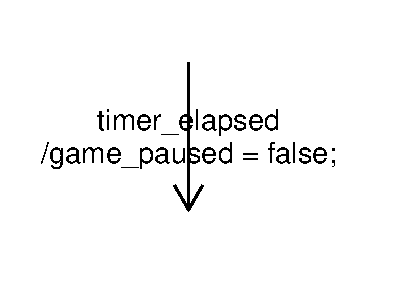
\includegraphics[scale=0.4]{../system_models/dynamic_models/menu_state_machine.pdf}
\caption{Zustandsautomat zur Menübedienung}
\end{figure}
%\restoregeometry

\begin{figure}[H]
\centering
\includegraphics[scale=0.55]{../system_models/dynamic_models/game_level_state_machine.pdf}
\caption{Zustandsautomat zum Ablauf eines Levels}
\end{figure}

\begin{figure}[H]
\centering
\includegraphics[scale=0.55]{../system_models/dynamic_models/reduction_mode_state_machine.pdf}
\caption{Zustandsautomat zur Funktion des Reduktions-Modus}
\end{figure}

\subsection{Benutzerschnittstelle}
%../GUI-Entwurf/_jpeg_numeration/registration1.gpej
%1-pflichtenheft/
\newcounter{B.SS}
\begin{figure}[H]

\centering
\refstepcounter{B.SS}\label{fig:Sprachauswahl}
\includegraphics[scale=0.55]{../GUI-Entwurf/_jpeg_numeration/registration1.jpg}

\caption{Sprachauswahl}


\end{figure}

\begin{figure}[H]
\centering
\refstepcounter{B.SS}\label{fig:Nameneingabe} 
\includegraphics[scale=0.55]
{../GUI-Entwurf/_jpeg_numeration/registration2.jpg}
\caption{Nameneingabe}
\end{figure}

\begin{figure}[H]
\centering
\refstepcounter{B.SS}\label{fig:Awatarauswahl}
\includegraphics[scale=0.55]{../GUI-Entwurf/_jpeg_numeration/registration3.jpg}
\caption{Awatarwahl}
\end{figure}

\begin{figure}[H]
\centering
\refstepcounter{B.SS}\label{fig:Profilauswahl}
\includegraphics[scale=0.55]{../GUI-Entwurf/_jpeg_numeration/choose_profile.jpg}
\caption{Profilauswahl}
\end{figure}

\begin{figure}[H]
\centering
\refstepcounter{B.SS}\label{fig:Welcome}
\includegraphics[scale=0.55]{../GUI-Entwurf/_jpeg_numeration/welcome.jpg}
\caption{Begrüssungsbildschirm}
\end{figure}

\begin{figure}[H]
\centering
\refstepcounter{B.SS}\label{fig:Hauptmenu}
\includegraphics[scale=0.55]{../GUI-Entwurf/_jpeg_numeration/main_manu.jpg}
\caption{Hauptmenu}
\end{figure}

\begin{figure}[H]
\centering
\refstepcounter{B.SS}\label{fig:Einstellungen}
\includegraphics[scale=0.55]{../GUI-Entwurf/_jpeg_numeration/settings.jpg}
\caption{Einstellungen}
\end{figure}

\begin{figure}[H]
\centering
\refstepcounter{B.SS}\label{fig:Status}
\includegraphics[scale=0.55]{../GUI-Entwurf/_jpeg_numeration/stat.jpg}
\caption{Status}
\end{figure}

\begin{figure}[H]
\centering
\refstepcounter{B.SS}\label{fig:achievments}
\includegraphics[scale=0.55]{../GUI-Entwurf/_jpeg_numeration/achievments.jpg}
\caption{Achievements}
\end{figure}

\begin{figure}[H]
\centering
\refstepcounter{B.SS}\label{fig:level}
\includegraphics[scale=0.55]{../GUI-Entwurf/_jpeg_numeration/level.jpg}
\caption{Levels}
\end{figure}

\begin{figure}[H]
\refstepcounter{B.SS}\label{fig:shop}
\centering
\includegraphics[scale=0.55]{../GUI-Entwurf/_jpeg_numeration/shop.jpg}
\caption{Shop}
\end{figure}

\begin{figure}[H]
\refstepcounter{B.SS}\label{fig:shop_popup}
\centering
\includegraphics[scale=0.55]{../GUI-Entwurf/_jpeg_numeration/shop_popup.jpg}
\caption{shoppopup}
\end{figure}







\section{Glossar}

\begin{description}
	\item[Achievement] \hfill \\
	Errungenschaft/Erfolg. Bezeichnet eine Auszeichnung für eine bestimmte Leistung.\\
	Kann im Spiel gewonnen werden.\\
	Beispiel: "Lambda für Anfänger" - Du hast das Tutorial erfolgreich abgeschlossen
	
	\item[Android] \hfill \\
	Betriebssystem und Softwareplattform hauptsächlich für mobile Geräte. Das Spiel/Produkt wird in erster Linie 
	für Android entwickelt.
	
	\item[App] \hfill \\
	Kurz für Application oder Applikation und bezeichnet Anwendungssoftware. Im Deutschen meistens jene von mobilen Geräten.
	
	\item[Avatar] \hfill \\
	Im Profil des Benutzers ist der Avatar, ein Bild, aus einer vorgefertigten Sammlung wählbar.
	Der Avatar soll, mit dem Profilnamen, den Nutzer repräsentiert und ist rein kosmetisch.
	Ziel ist dem Spieler die Möglichkeit zu geben sein Profil persönlicher gestalten.
	
	\item[Beta-Konversion] \hfill \\
	Stellt im Lambda-Kalkül das Konzept der Funktionsanwendung dar.
	
	\item[Checkbox] \hfill \\
	Ein Element grafischer Benutzeroberflächen. Wird meist als Kästchen dargestellt, das mit einem Klick aktiviert (abgehakt) oder
	wieder deaktiviert wird. Zum Beispiel um die Musik in einem Spiel an oder aus zu stellen.
	
	\item[Drag\&Drop-Geste] \hfill \\
	Der Benutzer klickt ein Objekt auf dem Bildschirm. Solange er nicht loslässt, "zieht" er das Objekt, wodurch
	es sich typischerweise mit seinem Finger mitbewegt. Lässt er los, lässt er das Objekt wieder "fallen", wodurch
	es an seinem neuen Platz abgelegt wird.
	
	\item[Editor] \hfill \\
	%TODO 
	
	\item[Lambda-Kalkül] \hfill \\
	Das Lambda-Kalkül ist eine formale Sprache, die zur Untersuchung von mathematischen Funktionen entwickelt wurde.
	Die Grundlagen des Lambda-Kalküls zu erlernen ist das Ziel des Produkts.
	
	\item[Level] \hfill \\
	Hier bezeichnet ein Level ein abgeschlossenen Teil des Spiels. Der Spieler betritt/startet das Level. Ihm wird eine Aufgabe,
	wie zum Beispiel ein Rätsel gestellt. Nach dem Abschließen der Aufgabe verlässt der Spieler das Level wieder.
	
	\item[Modus] \hfill \\
	%TODO
	
	\item[Münzen] \hfill \\
	Virtuelle Währung des Spiels. Sie kann zum Beispiel durch erfolgreiches Abschließen eines Levels verdient werden.
	Gewonnene Münzen können im Spiel dann wiederum ausgegeben werden.
	
	\item[Pinch-Geste] \hfill \\
	Durch Berührung zweier Punkte auf dem Bildschirm wird zwischen ihnen ein nicht sichtbares Zentrum erzeugt.
	Bewegt der Benutzer seine Finger näher zum Zentrum oder entfernt er sie weiter davon werden für gewöhnlich
	Aktionen wie die, entsprechend der Bewegung, Vergrößerung oder Verkleinerung von Objekten durchgeführt.
	
	\item[Popup] \hfill \\
	Popups sind kleinere Fenster, die auf dem Bildschirm erscheinen und das Fenster hinter ihnen teilweise verdecken.
	Sie zeigen oft zusätzliche Inhalte an oder suchen Bestätigung für eine Aktion des Nutzers.
	
	\item[Profil] \hfill \\
	Profile machen das Benutzen des Spiels von mehreren Personen möglich. Jeder Benutzer hat ein eigenes Profil,
	dass alle seine Daten (Name, Spielfortschritt usw.) speichert. Der Benutzer wählt beim Start sein Profil aus, wodurch das Spiel,
	wie er es zuvor verlassen hat, geladen wird, obwohl zum Beispiel in der Zwischenzeit ein Zweiter auf einem anderen Profil gespielt hat.
	
	\item[Reduktion] \hfill \\
	Oder Beta-Reduktion. Anderer Name für die Beta-Konversion, falls diese ausschließlich von links nach rechts angewandt wird.
	
	\item[Shop] \hfill \\
	Der Shop ist ein Menü im Spiel, indem die im Spiel existierende Währung der Münzen gegen verschiedenste Dinge eingetauscht werden kann.
	
	\item[Smartphone] \hfill \\
	Ein mobiles Telefon, dass mehr Computer-Funktionalitäten besitzt, als ein herkömmliches Telefon. Häufiges Merkmal ist ein sogenannter
	Touchscreen, der zu einem großen Teil zur Bedienung benutzt wird.
	
	\item[Tablet] \hfill \\
	Es ähnelt einem Smartphone und verwendet häufig auch für Smartphones entwickelte Betriebssysteme. 
	Ein Tablet ist aber normalerweise um ein Vielfaches größer und besitzt dadurch einen größeren Touchscreen.

	\item[Term] \hfill \\
	Mit einem Term wird hier ein Ausdruck im Lambda-Kalkül beschrieben. Das Spiel basiert auf der Idee solche Terme kindgerecht 
	zu visualisieren.
	
	\item[Touchscreen] \hfill \\
	Berührungsempfindlicher Bildschirm. Durch Berührungen und Gesten auf dem Touchscreen kann ein Gerät bedient werden.
	
	\item[Zoom] \hfill \\
	Durch Zoomen scheint Spieler den Bildausschnitt näher zu einem Objekt zu bewegen oder ihn weiter davon zu entfernen.
	Dadurch kann der Nutzer kleine Objekte größer darstellen oder sich bei vielen Objekten einen Überblick "von oben" verschaffen. 
\end{description}


\end{document}